\documentclass[11pt;a4paper]{report}
\usepackage[free-standing-units]{siunitx}
\usepackage{circuitikz}
\usepackage{tikz}
\usepackage[utf8]{inputenc}
\usepackage{fontenc}
\usepackage[french]{babel}
\usepackage{lmodern}
\usepackage{amsmath}
\usepackage{amssymb}
\usepackage{mathrsfs}
\usepackage[top=2cm, bottom=2cm, left=2cm, right=2cm]{geometry}
\usepackage{multirow}
\usepackage{url,hyperref}
\usepackage{siunitx}
\usepackage{schemabloc}
\usepackage{pgfplots}

\title{
\includegraphics{../../../images/inp-enseeiht} \\ ~ \\ ~ \\ ~ \\ ~ \\ Mini Projet Électronique Linéaire \\ ~ \\ \large{Réalisation d'un amplificateur de tension - rapport final}}
\author{Mathieu Morino, Guilhem Saurel}
\date{\oldstylenums{\today}}

%\renewcommand{\thechapter}{\Roman{chapter}}
%\renewcommand{\thechapter}{\thechapter .\Alph{chapter}}

\begin{document}
 \begin{titlepage}
  \maketitle
 \end{titlepage}

 \tableofcontents
 
 \chapter{Modifications apportées depuis le rapport intermédiaire}
  \section{Théorie}
    On ajoute un pont diviseur de tension en entrée afin de réduire l'amplitude du signal délivré par le générateur. En effet, celui-ci n'est pas capable de délivrer une tension de l'ordre du millivolt, nécessaire au fonctionnement du circuit. On choisi une réduction d'un facteur 100.

~

    On ajoute une résitance en parralèle à un "strap". Celui-ci court-circuité annule l'effet de la résistance placée à ses bornes et permet au circuit de fonctionner comme prévu. En outre, déconnecté, il permet d'effectuer des mesures d'impédance d'entrée.

~

    On ajoute une capacité de découplage entre Vcc et la masse, et ce pour chaque étage amplificateur, afin d'atténuer les parasites. On veillera à placer ces capacités le plus près possible des transistors lors du routage.

~

    On baisse la valeur de la résistance d'émetteur du dernier étage à 1k$\Omega$ afin de diminuer la distortion harmonique. En effet, celle-ci a une influence directe sur la pente de la droite de charge. 


  \section{Polarisations}
   \subsection{Premier étage : Collecteur commun}
    \begin{center}
     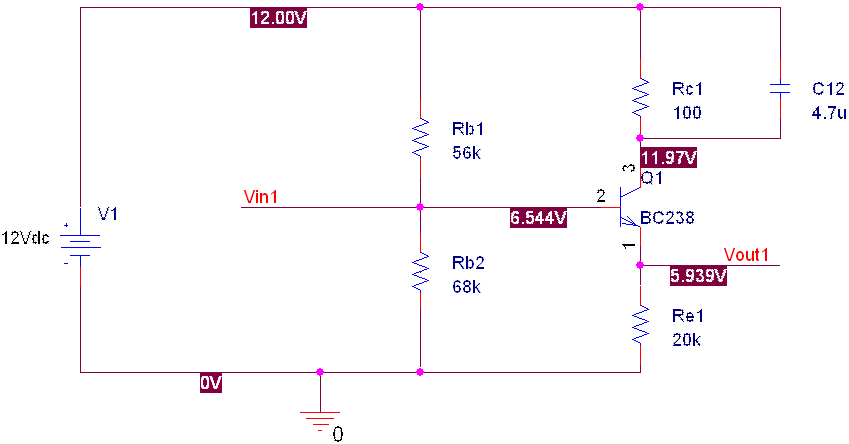
\includegraphics[width=17cm]{images/etage1.PNG}
    \end{center}

   \subsection{Deuxième étage : Émetteur commun}
    \begin{center}
     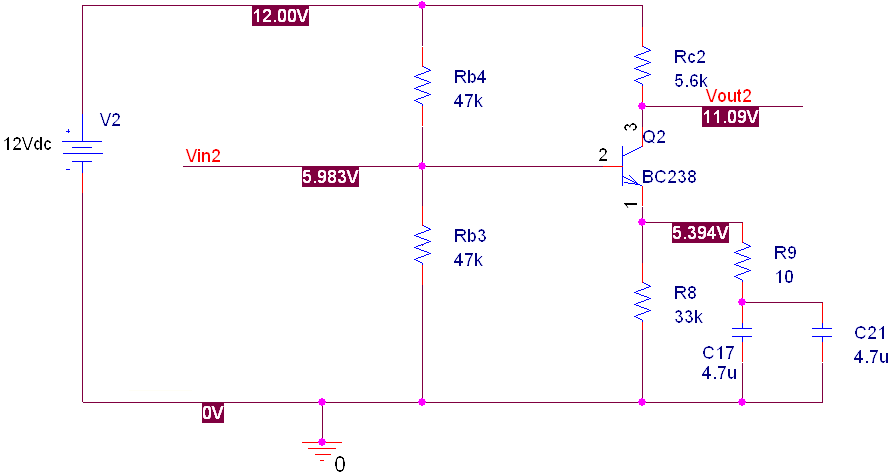
\includegraphics[width=17cm]{images/etage2.PNG}
    \end{center}

   \subsection{Troisième étage : Amplificateur différentiel}
    \begin{center}
     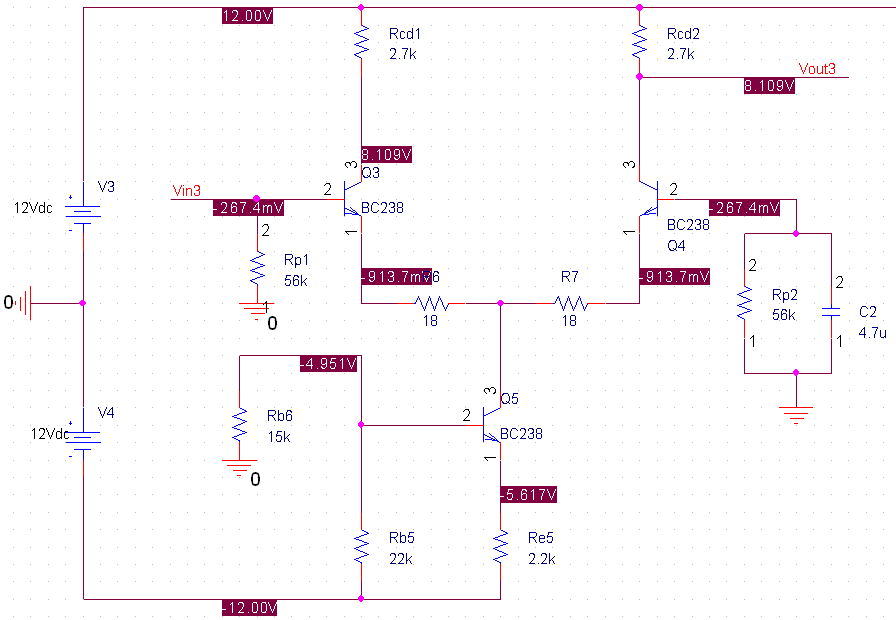
\includegraphics[width=17cm]{images/etage3.PNG}
    \end{center}

   \subsection{Quatrième étage : Collecteur commun}
    \begin{center}
     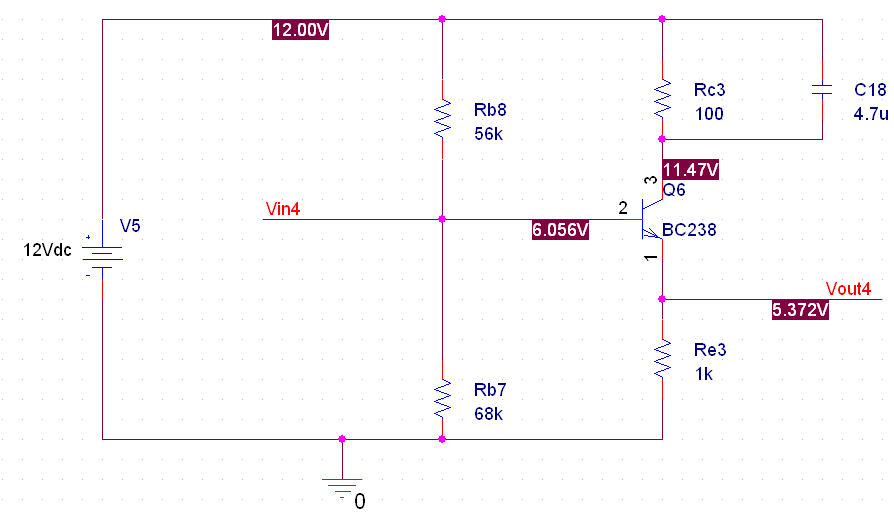
\includegraphics[width=17cm]{images/etage4.PNG}
    \end{center}

  \section{Schéma final}
   \begin{center}
    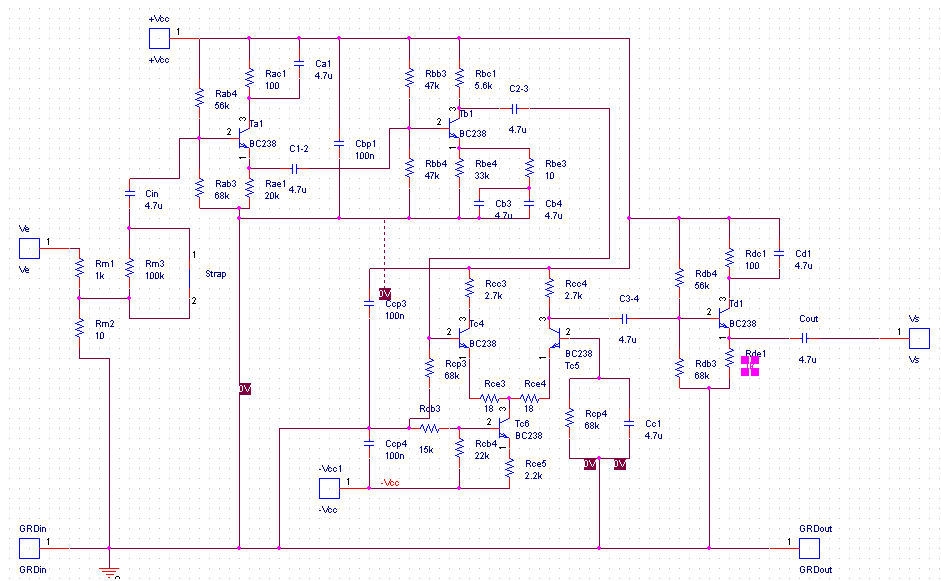
\includegraphics[height=14cm,angle=90]{images/projet1.PNG}
   \end{center}

 \chapter{Résultat du circuit sur plaquette LABDEC}
  \section{Deux premiers étages}
   \begin{center}
    \begin{tikzpicture}
     \begin{semilogxaxis}[width=17cm,height=10cm,xlabel=Fréquence (Hz),ylabel=Gain (dB)]
      \addplot[smooth]
       plot coordinates {
        (50,28.725)
        (100,29.363)
        (200,29.535)
        (300,29.535)
        (500,29.535)
        (1000,29.441)
        (2000,29.441)
        (3000,29.347)
        (5000,29.347)
        (10000,29.441)
        (20000,29.441)
        (30000,29.441)
        (50000,29.535)
        (100000,29.535)
        (200000,29.535)
        (300000,29.535)
        (500000,29.236)
        (1000000,28.415)
        (2000000,26.021)
        (3000000,19.046)
       };
     \end{semilogxaxis}
    \end{tikzpicture}
   \end{center}

   \begin{description}
    \item[Gain :]29.53 dB
    \item[Fréquence de coupure haute :]2 MHz
   \end{description}

  \section{Circuit complet}
   \begin{center}
    \begin{tikzpicture}
     \begin{semilogxaxis}[width=17cm,height=10cm,xlabel=Fréquence (Hz),ylabel=Gain (dB)]
      \addplot[smooth]
       plot coordinates {
        (1,50.962)
        (2,54.158)
        (3,55.455)
        (5,55.663)
        (10,55.757)
        (20,55.958)
        (30,55.958)
        (50,55.958)
        (100,55.958)
        (200,55.958)
        (300,55.958)
        (500,55.958)
        (1000,55.760)
        (2000,55.567)
        (3000,54.615)
        (5000,53.164)
        (10000,50.028)
        (20000,44.818)
        (30000,38.697)
        (50000,34.260)
       };
     \end{semilogxaxis}
    \end{tikzpicture}
   \end{center}

   \begin{description}
    \item[Gain :]55.96 dB
    \item[Fréquence de coupure basse :]71 Hz
    \item[Fréquence de coupure haute :]310 kHz
   \end{description}
 
 \chapter{Routage}
  \begin{center}
   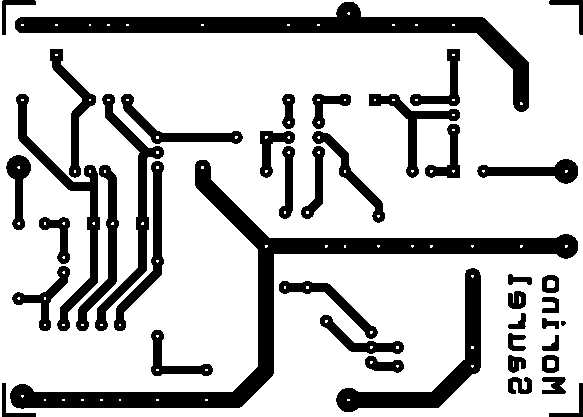
\includegraphics{images/layout} %TODO a mettre au milieu.
  \end{center}

 \chapter{Résultat du montage}
  \section{Deux premiers étages}
   \begin{description}
    \item[Gain :]25 dB
    \item[Fréquence de coupure basse :]100 Hz
    \item[Fréquence de coupure haute :]3 MHz
   \end{description}

  \section{Trois premiers étages}
   \begin{description}
    \item[Gain :]57.99 dB
    \item[Fréquence de coupure basse :]93 Hz
    \item[Fréquence de coupure haute :]504 kHz
   \end{description}

  \section{Circuit complet}
   \begin{description}
    \item[Gain :]56.81  dB
    \item[Fréquence de coupure basse :]85 Hz
    \item[Fréquence de coupure haute :]550 kHz
   \end{description}

  \section{Vérification des tensions de polarisation}
   \begin{center}
    \begin{tabular}{|l|l|c|c|}
     \hline
     \multicolumn{2}{|c|}{Lieu de la mesure} & Tension théorique & Tension obtenue \\
     \hline
     \multirow{3}{3cm}{Premier étage} & 
     Base  & 6.544 V & 6.375 V \\
     \cline{2-4} &
     Collecteur & 11.97 V & 11.86 V \\
     \cline{2-4} &
     Emetteur & 5.939 V & 5.74 V \\
     \hline
     \multirow{3}{3cm}{Deuxième étage} & 
     Base & 5.983 V & 5.97 V \\
     \cline{2-4} &
     Collecteur & 11.09 V & 11.25 V \\
     \cline{2-4} &
     Emetteur & 5.394 V & 5.71 V \\
     \hline
     \multirow{3}{3cm}{Troisième étage} & 
     Base & -267.4 mV & -198 mV \& -241 mV\\
     \cline{2-4} &
     Collecteur & 9.109 V & 9.15 V \& 7.68 V \\
     \cline{2-4} &
     Emetteur & -913mV & -776mV \& -776mV  \\
     \hline
     \multirow{3}{3cm}{Source de courant} & 
     Base & -4.951V & -4.8 V\\
     \cline{2-4} &
     Collecteur & & -790mV \\
     \cline{2-4} &
     Emetteur & -5.817mV & -5.51 mV\\
     \hline
     \multirow{3}{3cm}{Quatrième étage} & 
     Base & 6.056 V & 6.3 V \\
     \cline{2-4} &
     Collecteur & 11.47 V & 11.6 V \\
     \cline{2-4} &
     Emetteur & 5.372 V & 5.6V  \\
     \hline
    \end{tabular}
   \end{center}

  \section{Diagramme de Bode final}
   \begin{center}
    \begin{tikzpicture}
     \begin{semilogxaxis}[width=17cm,height=10cm,xlabel=Fréquence (Hz),ylabel=Gain (dB)]
      \addplot[smooth]
       plot coordinates {
        (50,50.87)
        (100,54.51)
        (200,56.17)
        (300,56.48)
        (500,56.68)
        (1000,56.78)
        (2000,56.76)
        (3000,56.76)
        (5000,56.77)
        (10000,56.77)
        (20000,56.77)
        (30000,56.86)
        (50000,56.71)
        (100000,56.53)
        (200000,55.87)
        (300000,55.77)
        (500000,54.08)
        (1000000,41.21)
        (2000000,38.76)
        (3000000,34.89)
        (5000000,30.14)
       };
     \end{semilogxaxis}
    \end{tikzpicture}
   \end{center}



 \chapter{Respect du cahier des charges} % TODO
  \begin{tabular}{|l|l|c|c|c|c|c|c|c|}
   \hline
   & & & Min & Max & Unit. & Sim. & Labdec & Circuit \\
   \hline
   \multirow{4}{3cm}{Caractéristiques générales à 30k\hertz} & Gain en tension & 60 & 55 & 65 & dB & \textcolor{green}{57.95} & \textcolor{green}{55.96} & \textcolor{green}{57.99} \\
   \cline{2-9} & Résistance d'entrée & 30 & 25.5 & 34.5 & \kilo\ohm & \textcolor{green}{29.658} & &  \textcolor{red}{36.111}  \\
   \cline{2-9} & Résistance de sortie & 100 & 85 & 115 & \ohm & \textcolor{green}{113} & & \textcolor{green}{82} \\
   \cline{2-9} & Dynamique de sortie & & 6 & & V càc & \textcolor{red}{5.98} & &  \textcolor{red}{5.98} \\
   \hline
   \multirow{2}{3cm}{Fréquence de coupure} & basse & 100 & 80 & 120 & \hertz & \textcolor{green}{101} & \textcolor{red}{71} & \textcolor{green}{93}\\
   \cline{2-9} & haute & & 500 & & k\hertz & \textcolor{green}{504} & \textcolor{red}{310} & \textcolor{green}{504} \\
   \hline
   Distorsion harmonique & [1k\hertz;100k\hertz] & & & 1,00 & \% & \textcolor{red}{6.003}&  & \textcolor{red}{6.1}\\
   \hline
   \multirow{2}*{Tension d'alimentation} & Positive & 12V & 0 & 12 & V & 12 & 12 & 12\\
   \cline{2-9} & Négative & -12V & -12 & 0 & V & -12 & -12 & -12\\
   \hline
   Courant de collecteur & & & 0.1 & 10 & mA & OK & & 12 mA (total)\\
   \hline
  \end{tabular}

  \subsection{Remarque}
   Notre fréquence de coupure haute correspond au cahier des charges juste parce qu'on a de la chance. S'il avait fallu l'augmenter, on aurait pu modifier la symétrie de l'amplificateur différentiel en augmentant la résistance sur le collecteur du transistor en entrée. Cette dissymétrie aurait eu très peu d'impact, et si on baisse cette résistance, on augmente la fréquence de coupure haute la plus basse de notre circuit ( cette dernière est en effet dûe à l'effet miller, donc augmenter la résistance augmente la constante de temps du passe-bas engendré par cet effet Miller).

  \chapter{Photos}
   \begin{center}
    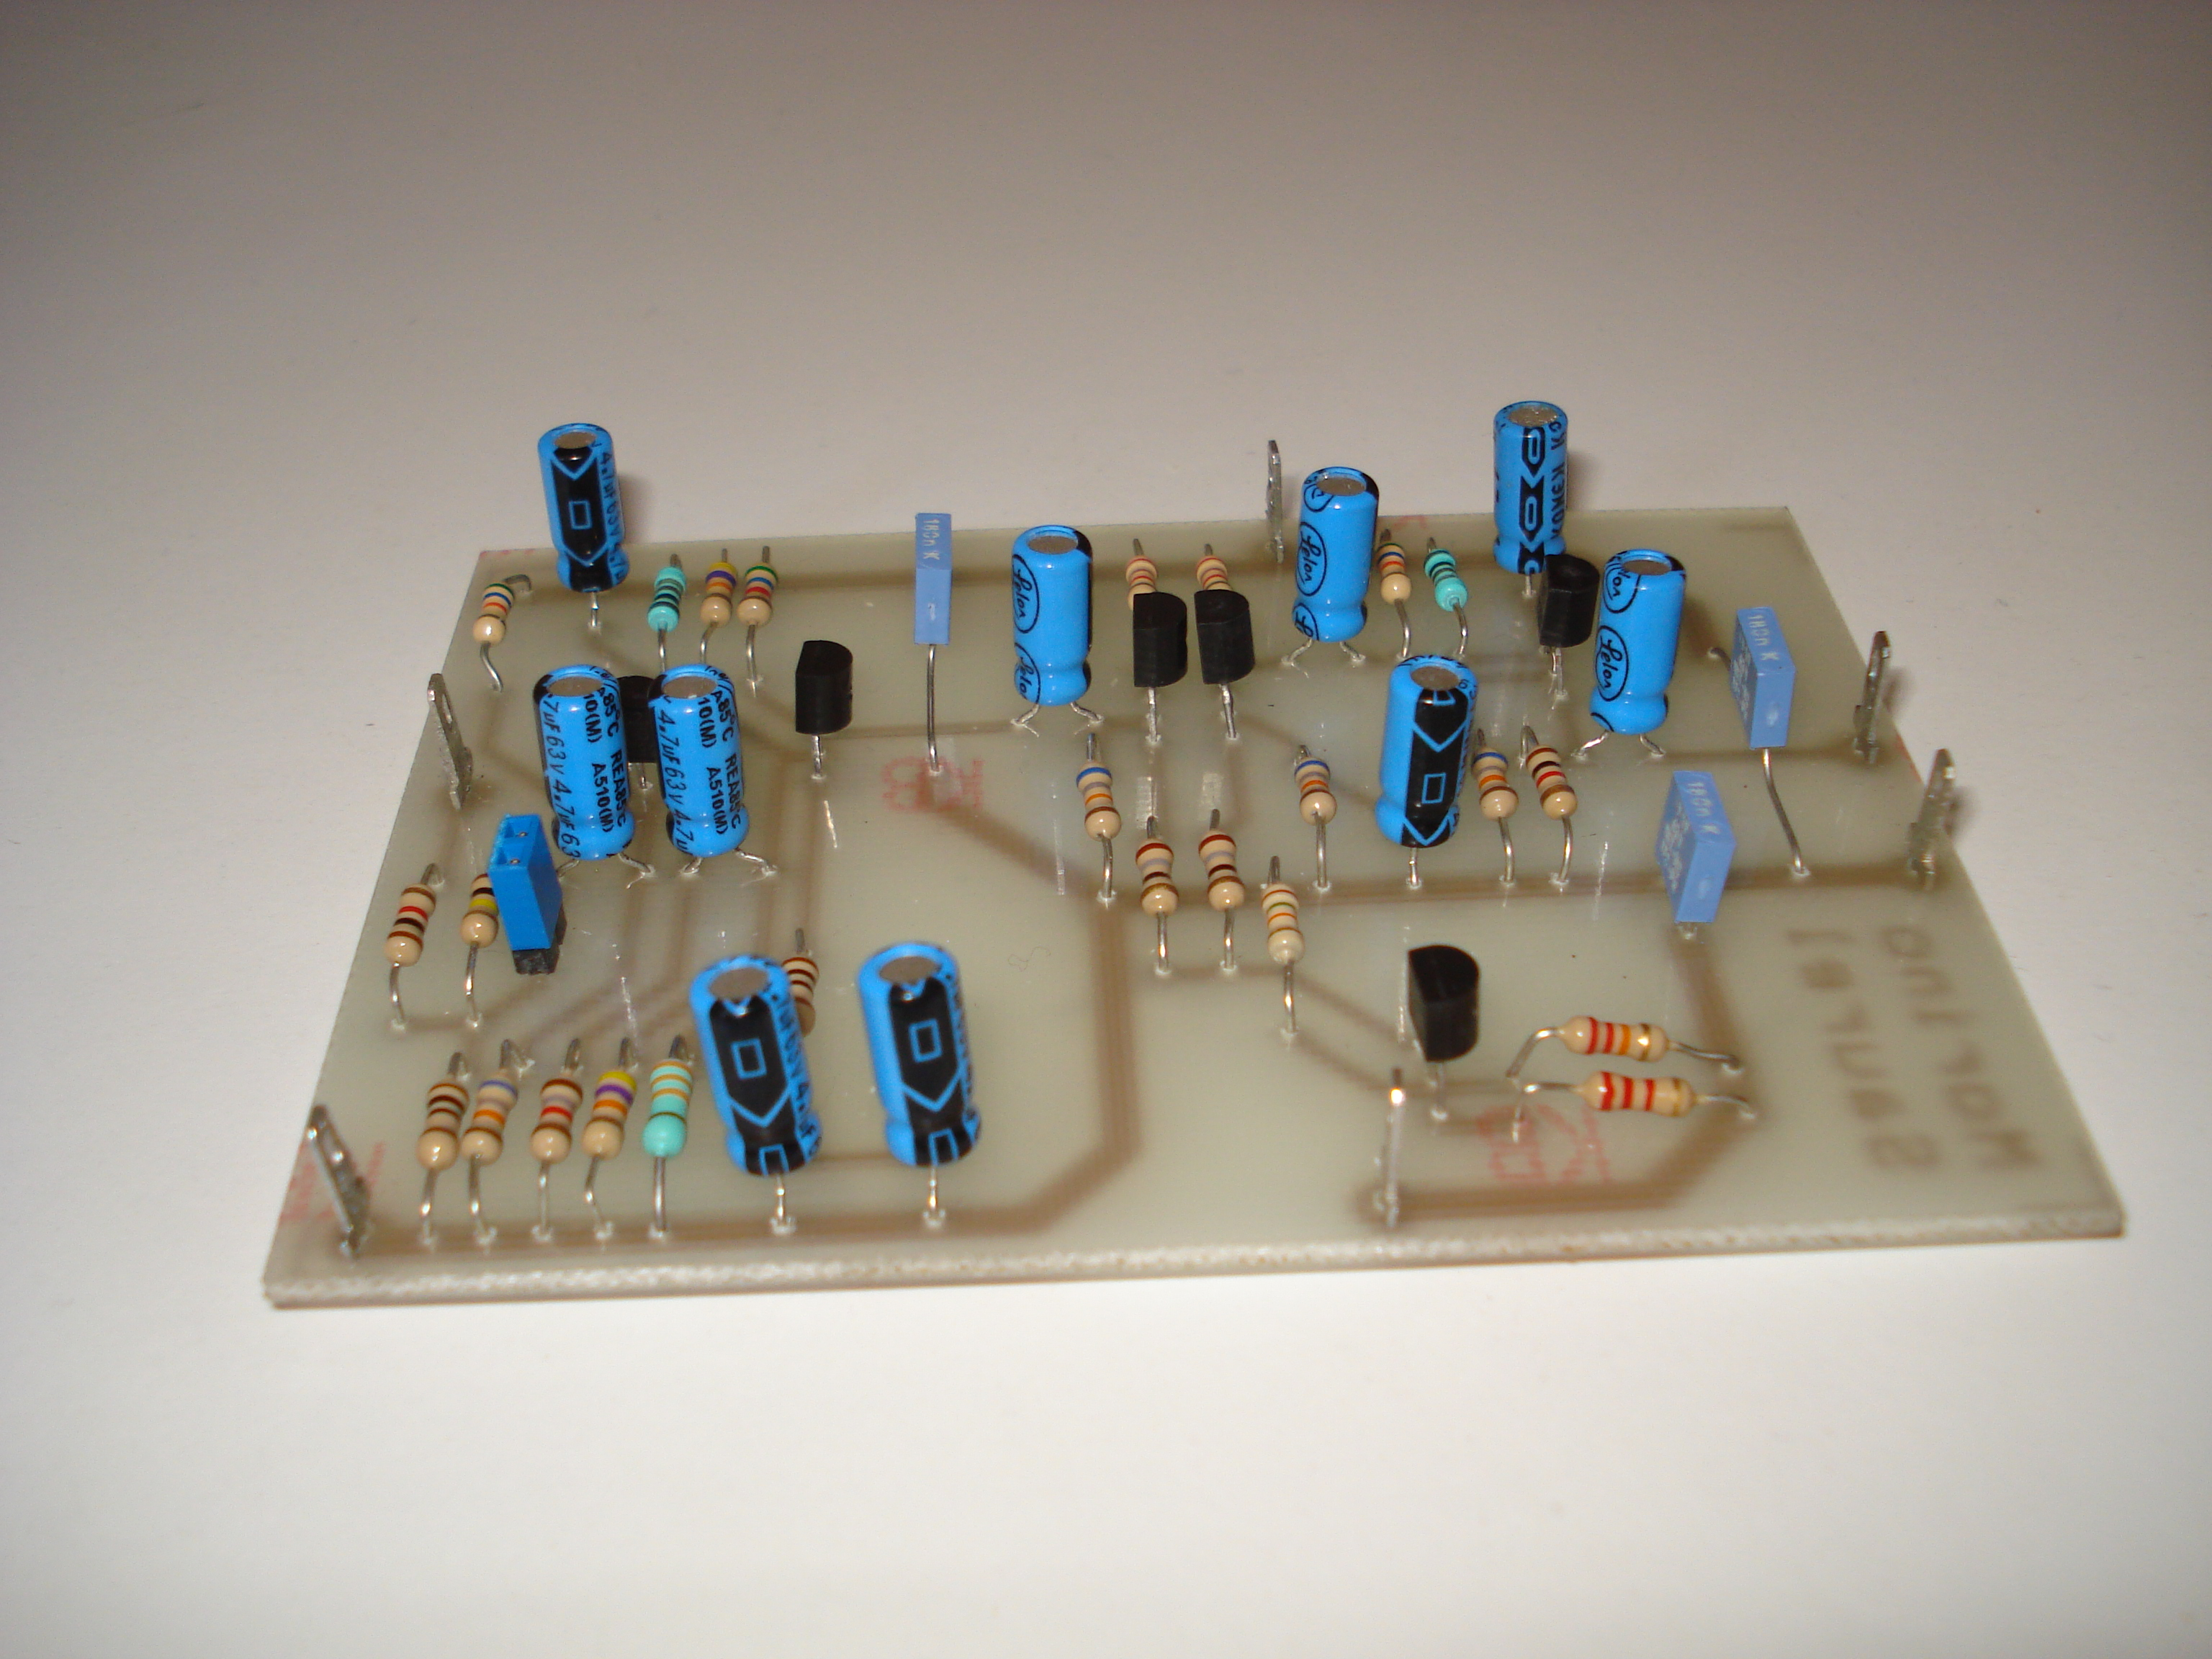
\includegraphics[width=\linewidth]{images/recto}

    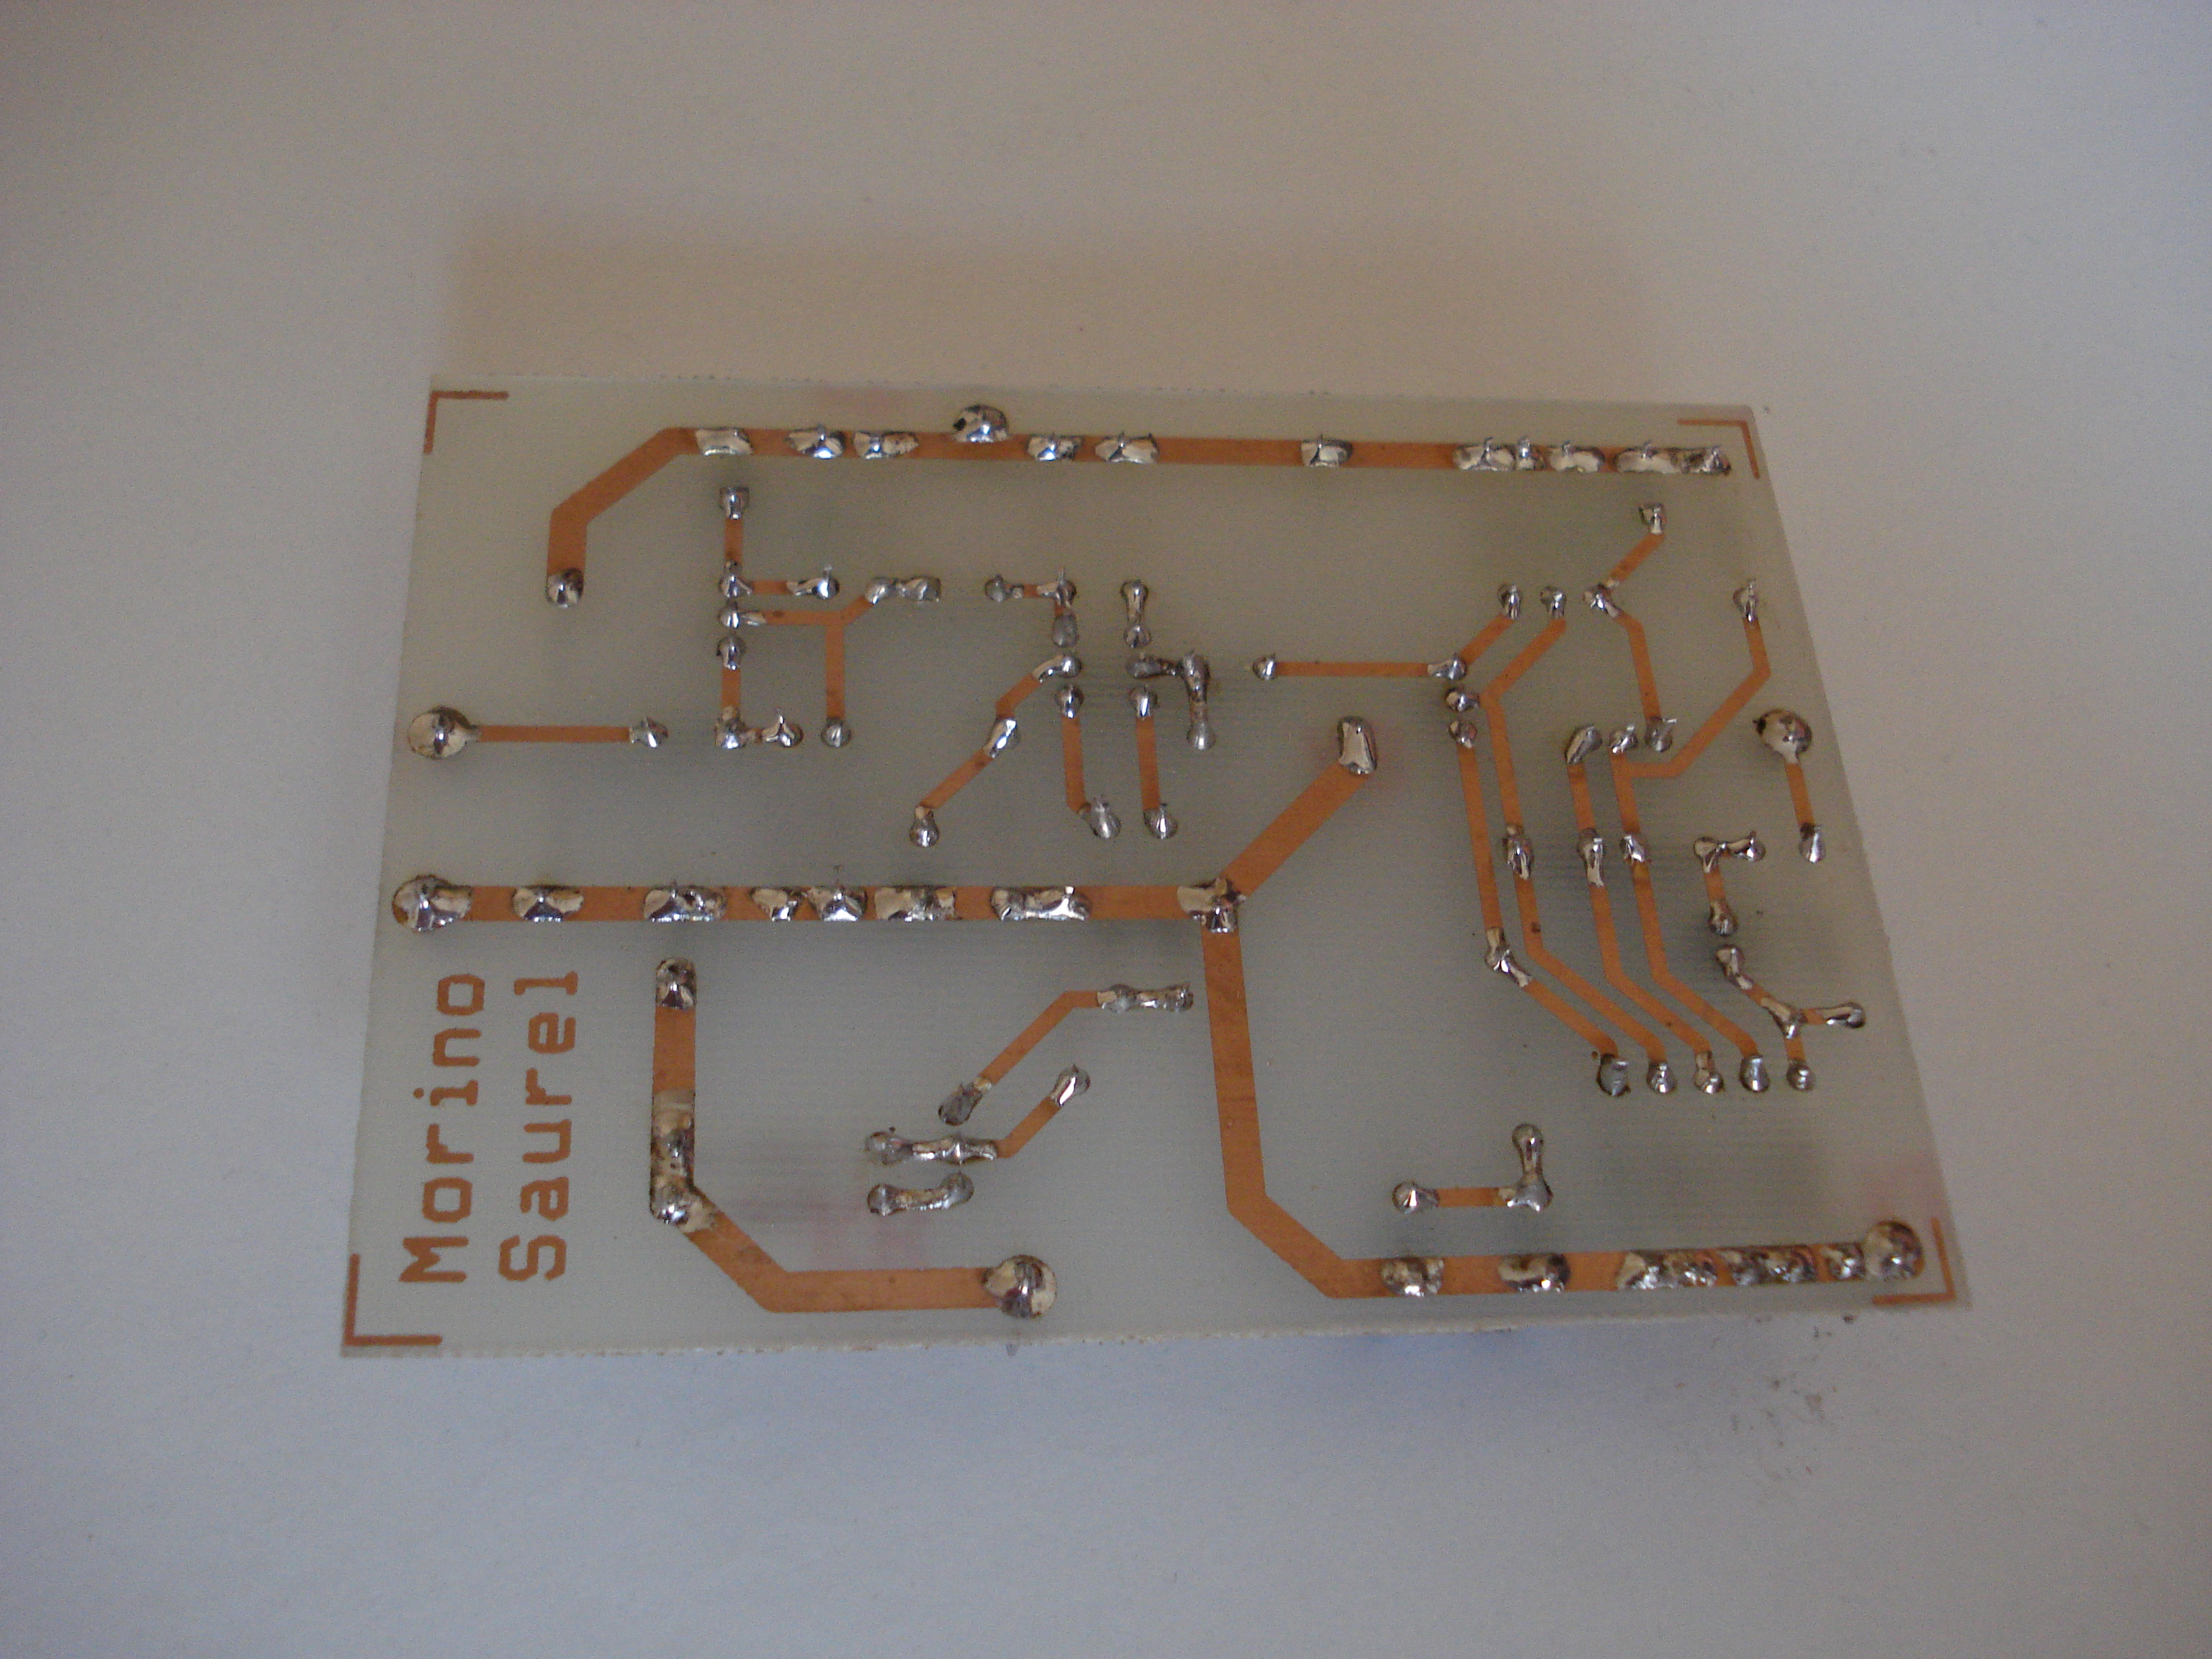
\includegraphics[width=\linewidth]{images/verso}
   \end{center}

\end{document}
